% DBPU top-level architecture (matches rtl/branch_prediction_top.v)
% Build: cd docs/diagrams && tectonic dbpu_architecture.tex
\documentclass[tikz,border=8pt]{standalone}
\usetikzlibrary{arrows.meta,positioning,fit,backgrounds,calc}
\begin{document}
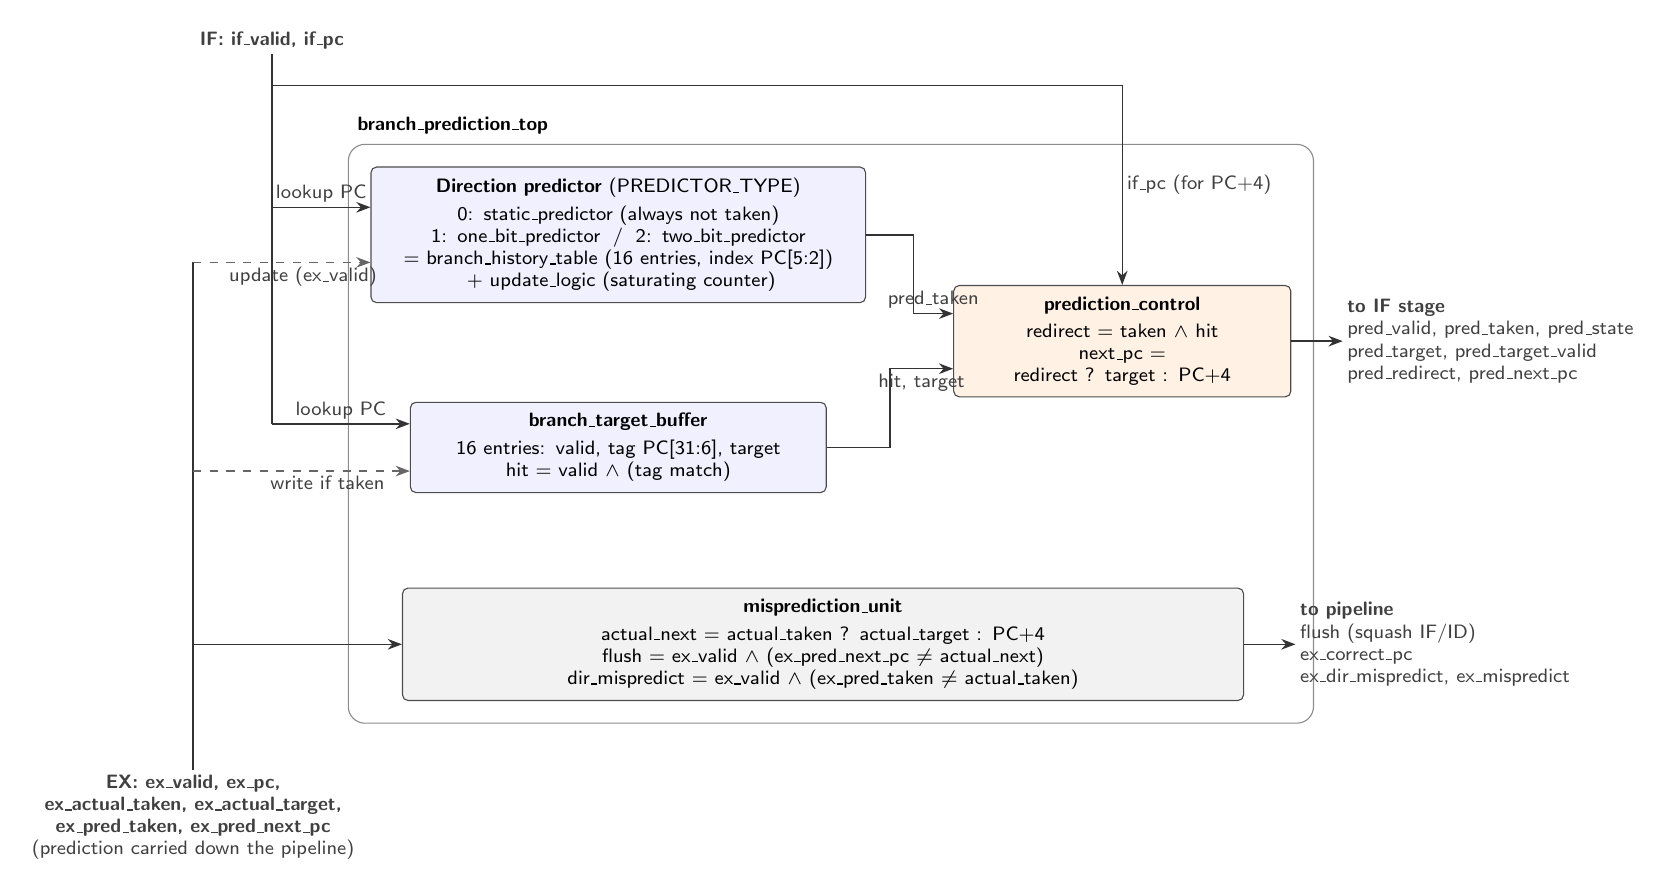
\begin{tikzpicture}[
  font=\sffamily\scriptsize, >={Stealth[length=1.8mm]},
  blk/.style={draw=black!70, rounded corners=2pt, fill=#1, align=center, inner sep=4pt},
  blk/.default=white,
  sig/.style={->, draw=black!80, line width=0.5pt},
  upd/.style={->, draw=black!60, line width=0.5pt, dashed},
  lbl/.style={font=\sffamily\scriptsize, text=black!75, inner sep=1.5pt}
]
% ---------------- blocks ----------------
\node[blk=blue!6, text width=60mm] (pred) at (0,0)
  {\textbf{Direction predictor} (PREDICTOR\_TYPE)\\[2pt]
   0: static\_predictor (always not taken)\\
   1: one\_bit\_predictor \;/\; 2: two\_bit\_predictor\\
   = branch\_history\_table (16 entries, index PC[5:2])\\
   \;+ update\_logic (saturating counter)};
\node[blk=blue!6, text width=50mm] (btb) at (0,-2.7)
  {\textbf{branch\_target\_buffer}\\[2pt] 16 entries: valid, tag PC[31:6], target\\ hit = valid $\wedge$ (tag match)};
\node[blk=orange!10, text width=40mm] (pc) at (6.4,-1.35)
  {\textbf{prediction\_control}\\[2pt] redirect = taken $\wedge$ hit\\ next\_pc =\\ \mbox{redirect ? target : PC+4}};
\node[blk=black!5, text width=104mm] (mp) at (2.6,-5.2)
  {\textbf{misprediction\_unit}\\[2pt] actual\_next = actual\_taken ? actual\_target : PC+4\\
   \mbox{flush = ex\_valid $\wedge$ (ex\_pred\_next\_pc $\neq$ actual\_next)}\\ \mbox{dir\_mispredict = ex\_valid $\wedge$ (ex\_pred\_taken $\neq$ actual\_taken)}};

% ---------------- IF bus ----------------
\coordinate (ifb) at (-4.4,2.3);
\node[lbl, anchor=south, font=\sffamily\scriptsize\bfseries] at (ifb) {IF: if\_valid, if\_pc};
\draw[line width=0.5pt, black!80] (ifb) -- (-4.4,-2.4);
\draw[sig] (-4.4,0.35) -- node[lbl,above]{lookup PC} (pred.west |- 0,0.35);
\draw[sig] (-4.4,-2.4) -- node[lbl,above]{lookup PC} (btb.west |- 0,-2.4);
\draw[sig] (-4.4,1.9) -- (6.4,1.9) -- node[lbl,right]{if\_pc (for PC+4)} (pc.north);

% ---------------- EX bus ----------------
\coordinate (exb) at (-5.4,-6.8);
\node[lbl, anchor=north, align=center, font=\sffamily\scriptsize\bfseries] at (exb)
  {EX: ex\_valid, ex\_pc,\\ ex\_actual\_taken, ex\_actual\_target,\\ ex\_pred\_taken, ex\_pred\_next\_pc\\ \mdseries(prediction carried down the pipeline)};
\draw[line width=0.5pt, black!80] (exb) -- (-5.4,-0.35);
\draw[upd] (-5.4,-0.35) -- node[lbl,below, pos=0.62]{update (ex\_valid)} (pred.west |- 0,-0.35);
\draw[upd] (-5.4,-3.0) -- node[lbl,below, pos=0.62]{write if taken} (btb.west |- 0,-3.0);
\draw[sig] (-5.4,-5.2) -- (mp.west);

% ---------------- internal ----------------
\draw[sig] (pred.east) -- (3.75,0) |- node[lbl,above, pos=0.75]{pred\_taken} ($(pc.west)+(0,0.35)$);
\draw[sig] (btb.east) -- (3.45,-2.7) |- node[lbl,below, pos=0.75]{hit, target} ($(pc.west)+(0,-0.35)$);

% ---------------- outputs ----------------
\node[lbl, anchor=west, align=left] (ifout) at (9.2,-1.35)
  {\textbf{to IF stage}\\ pred\_valid, pred\_taken, pred\_state\\ pred\_target, pred\_target\_valid\\ pred\_redirect, pred\_next\_pc};
\draw[sig] (pc.east) -- (ifout.west);
\node[lbl, anchor=west, align=left] (exout) at (8.6,-5.2)
  {\textbf{to pipeline}\\ flush (squash IF/ID)\\ ex\_correct\_pc\\ ex\_dir\_mispredict, ex\_mispredict};
\draw[sig] (mp.east) -- (exout.west);

\begin{scope}[on background layer]
  \node[draw=black!45, rounded corners=6pt, fit=(pred)(btb)(pc)(mp), inner sep=8pt,
        label={[font=\sffamily\scriptsize\bfseries, anchor=south west]north west:branch\_prediction\_top}] {};
\end{scope}
\end{tikzpicture}
\end{document}
